\chapter{Evaluation of process fusion}
\label{s:Benchmarks}
Stream fusion is ultimately performed for practical reasons: we want the fused result program to run faster than the original unfused program.
We also need to be sure that the fused program is not too large, to ensure that compilation and the fusion transform do not consume too much memory.
This chapter shows runtime benchmark results for fused programs, and the result size of fused programs.

\section{Benchmarks}

The process fusion algorithm described in \cref{chapter:process:processes} is implemented in a library called \emph{Folderol}\footnote{\url{https://github.com/amosr/folderol}}.
% To benchmark our algorithm, we have implemented the fusion algorithm described in \cref{chapter:process:processes}, in a library called \emph{Folderol}\footnote{\url{https://github.com/amosr/folderol}}.
Our implementation uses the topology of the entire process network to perform fusion, statically coordinating between all processes in the network.
To fuse the entire process network at compile-time, Folderol uses Template Haskell, a form of metaprogramming.

\newcommand\Streaming[0] {{\sc Streaming}\xspace}
% For the benchmarks, We use the \emph{Folderol} Template Haskell implementation. % described in \cref{chapter:process:implementation}.
Benchmarks are available at \url{https://github.com/amosr/folderol/tree/master/bench}.
As well as the ``gold panning'' example from \cref{taxonomy/gold-panning}, we present one spatial algorithm, two file-based benchmarks, and one audio signal processing benchmark.
In the benchmarks, we compare Folderol variously against hand-fused implementations, the array library Vector \cite{hackage:vector}, as well as streaming libraries Conduit \cite{hackage:conduit}, Pipes \cite{hackage:pipes} and \Streaming\footnote{We use this typography to distinguish \Streaming the library from streaming the abstract concept.} \cite{hackage:streaming}.
We restrict our attention to Haskell libraries to isolate the cost of streaming from language implementation details.
The concepts in the chosen libraries are applicable to other languages, and we expect other implementations to show comparable benchmark results.
Strymonas \citep{kiselyov2016stream}, which has OCaml and Scala implementations, uses a similar stream representation to Vector, but uses staged computation to perform fusion.
Functional streams for Scala \citep{package:scala:fs2} uses a similar representation to Pipes and Conduit.


The Vector library provides high-performance boxed and unboxed arrays with pull-based shortcut fusion.
It is the \emph{de facto} standard for array programming in Haskell, and implements a shortcut fusion system called \emph{stream fusion}, introduced by \citet{coutts2007stream}.
Array operations are implemented by converting the input array to a stream, then performing the corresponding stream operation, and converting back to an array.
The shortcut fusion rule removes the superfluous conversion when a stream is converted to an intermediate array and immediately back to a stream.
Just as pull streams only support a single consumer, this rule can only remove intermediate arrays which have a single consumer.
If the same intermediate array is used multiple times, it acts as a \emph{fusion barrier}, forcing the stream to be manifested into a real, memory-backed array.
We discuss fusion barriers further in \cref{clustering}.
% While the fusion is pull-based, splits can still be expressed in the program by mentioning the same array multiple times.
% These splits act as fusion barriers, requiring streams to be manifested as in-memory arrays.
In practice, Vector provides no guarantees about whether fusion will occur, and the easiest way to tell whether fusion has occurred is to look at the generated code to count the loops and arrays.
We could benchmark the program to see whether it is ``fast enough'', but if we do not have an optimal baseline to compare against, it is hard to know how fast the program \emph{should} be.
After inspecting the generated code, if we discover that fusion has not occurred, it may be necessary to rewrite the program and hand-fuse it.
% it is a different thing to convince the compiler to somehow fuse it: perhaps the program must be rewritten and hand-fused, or perhaps strictness annotations are required.

% \TODO{Move elsewhere.}
% The Stream part of Vector is split into two types: the fully general stream, which is parameterised over a monad, and pure streams, essentially specialised to the identity monad.
% Vector has a minor problem with monadic actions, but this is an implementation detail that could probably be ignored.
% Converting from monadic streams back to vectors goes via linked-lists: this is because constructing a vector requires \Hs@ST@ or \Hs@IO@, but we cannot easily interleave the stream's monadic actions (which may be an arbitrary monad) with effects from \Hs@IO@.
% Instead, the current implementation runs all of the stream's actions, collecting the result in a list, and only constructs the vector after the stream has finished.
% This way, the effects do not need to be interleaved.
% It is possible to write this using several unsafe operations, but one must be \emph{very} careful for this, taking into account that laziness must be conquered to ensure the correct interleaving.

The first two Haskell streaming libraries, Conduit and Pipes, both have limited APIs that ensure that any computation can be run with bounded buffers.
These streaming libraries do not naturally support multiple queries: when a stream is shared among multiple consumers, part of the program must be hand-fused, or somehow rewritten as a straight-line computation.
These libraries also have a monadic interface, which allows the structure of the dataflow graph to depend on the values.
This expressiveness has a price: if the dataflow graph can change dynamically, we cannot statically fuse it.
% This price is paid even when the dataflow graph is static, as the same monadic structure is used: because repetition is expressed as an unfolding dynamic graph, even computations that would be static in other systems must be expressed dynamically, reducing the possibility for fusion.

\begin{haskell}[float,caption=Conduit datatypes,label=l:bench:def:conduit]
data ConduitT i o m r =
    NeedInput  (i -> ConduitT i o m r) (ConduitT i o m r)
  | HaveOutput (ConduitT i o m r) o
  | Done r
  | ConduitM   (m (ConduitT i o m r))
  | Leftover   (ConduitT i o m r) i

instance Monad m => Monad (ConduitT i o m)
\end{haskell}

\Cref{l:bench:def:conduit} shows a simplified version of the core datatype for Conduit.
The \Hs/ConduitT/ type defines a stream transformer that consumes elements of type \Hs/i/ and produces elements of type \Hs/o/.
The transformer may perform effects in the \Hs/m/ monad, and returns a final result value of type \Hs/r/.
The \Hs/NeedInput/ constructor pulls from the input and takes two arguments: a function which takes the input element and returns a new stream transformer, and a stream transformer to use when the input stream is finished.
The \Hs/ConduitM/ constructor performs a monadic effect, which returns a new stream transformer for the rest of the stream.
Because the data structure describing remainder of the stream is nested inside a closure that performs a monadic computation, the compiler may not be able to statically reason about the remainder of the stream.
The constructors and closures for the remainder of the stream will be allocated at runtime, instead of being statically optimised away.
To reduce this overhead, Conduit also implements a fusion system based on Vector's stream fusion \citep{coutts2007stream}.
In stream fusion, the stream is decomposed into a static, non-recursive step function and a dynamic state.
The static, non-recursive step function is simpler to inline and optimise than the recursive structure.
Many of the combinators are implemented in terms of both stream fusion as well as the Conduit implementation.
Rewrite rules are used to replace the Conduit implementation with the stream fusion implementation where possible.
Some Conduit operations, such as monadic bind, cannot be efficiently implemented in terms of stream fusion, because the structure of the stream can dynamically depend on the bound value.

The Pipes library uses a recursive, monadic data structure to represent stream transformers.
This representation is similar to the representation used by Conduit, and involves similar runtime overhead.
Instead of using stream fusion, Pipes has an extensive set of rewrite rules to statically optimise particular sequences of operations.

% In stream fusion, the stream is represented as a static step function and a dynamic state.
% Vector's static step function can be optimised at compile-time, while the state can change dynamically.
% In contrast, in Conduit and Pipes, the step function and state are mixed together: the remainder of the stream is only available dynamically as a function closure, hidden inside the continuation for a monadic operation.

\begin{haskell}[float,caption=\Streaming library datatypes,label=l:bench:def:streaming]
data Stream f m r =
    Step   (f (Stream f m r))
  | Effect (m (Stream f m r))
  | Return r
instance (Functor f, Monad m) => Monad (Stream f m)

data Of a b = a :> b
instance Functor (Of a)

store :: Monad m =>
      (Stream (Of a) (Stream (Of a) m) r -> t) ->
      Stream (Of a) m r -> t

sum  :: (Num a, Monad m) =>
      Stream (Of a) m r -> m (Of a r)
\end{haskell}

The \Streaming library is a monadic streaming library, similar to Conduit and Pipes.
\Cref{l:bench:def:streaming} shows the core datatypes for \Streaming.
The \Hs/Stream/ type defines a stream producer parameterised by a functor \Hs/f/, a monad \Hs/m/, and a result type \Hs/r/.
The functor for a stream producer is often instantiated to (\Hs/Of a/), where \Hs/a/ is the type of the producer's stream elements.
When the functor is instantiated to (\Hs/Of a/), the \Hs/Step/ constructor for \Hs/Stream/ will contain the produced stream element of type \Hs/a/, as well as the remaining stream.
The \Hs/Effect/ constructor, like the \Hs/ConduitM/ constructor in Conduit, performs an effect and returns the remaining stream.
The \Hs/Return/ constructor signals the end of the stream, and returns the result \Hs/r/.
\Streaming can execute multiple queries by explicitly duplicating streams, similar to polarised streams (\cref{taxonomy/polarised}).
To duplicate the stream, the \Hs@store@ function takes a computation to perform on the copy of the stream.
This operation is analogous to the \Hs/dup_ioi/ combinator, which duplicates a pull stream into a push stream and returns a new pull stream; however, the implementation encodes stream polarity with a monad transformer stack rather than directly using pull and push streams.
The computation passed to \Hs/store/ is a function that takes a \Hs/Stream/ representing the duplicated stream, with the original stream nested inside the monad transformer stack.
We can sum the elements of the duplicated stream while passing through the original elements like so:
\begin{haskell}
store sum :: Num a => Stream (Of a) m r -> Stream (Of a) m (Of a r)
\end{haskell}

The input stream has the result type \Hs/r/, while the modified stream contains the same elements and has the result type (\Hs/Of a r/), which is effectively a pair of the sum and the original result.
By putting the original stream in the duplicated stream's monad transformer stack, the original stream's elements are encoded as effects to be performed by the sum computation, while it pulls from the duplicated stream.
Unfortunately, because each stream element involves constructing the \Hs/Stream/ recursive data structure with a stack of monad transformers, the corresponding runtime allocations and closures are not always statically optimised away.

The benchmark results presented in this chapter were all run on a MacBook Pro, with a 2GHz Intel Core i7, and 16GB of RAM.
The operating system is OS X El Capitan with Glasgow Haskell Compiler (GHC) 8.0.2.
To run the benchmarks, we used the Criterion\footnote{\url{http://hackage.haskell.org/package/criterion}} library.
Criterion offers a fairly reliable way to evaluate runtime performance, as it runs each benchmark multiple times to compute the mean runtime, and warns if the variance is too high or if there are outliers.
It can also collect statistics on allocations, which can be a more stable performance indicator than runtime, as it is less affected by the underlying operating system's scheduling decisions.

We have implemented each benchmark program multiple times across the different backends.
These different implementations generally follow the same structure.
All the implementations are available in \cref{app:Benchmarks}; in this chapter, we focus on the Folderol versions.
% Showing five different implementations of the same program is not that interesting.
% For the most part, we show only the implementations of the Folderol versions; the other versions are available in \cref{app:Benchmarks}.

\subsection{Gold panning}

Our first benchmark is the \Hs@priceAnalyses@ example from \cref{taxonomy/gold-panning}.
This example computes statistical analyses of a particular stock's price over time, as well as how the stock compares to a market index.

\begin{haskell}[float,caption=Folderol implementation of \Hs/priceAnalyses/,label=l:bench:priceAnalysesFolderol]
priceAnalysesFolderol :: (FilePath,FilePath) -> IO (Double,Double)
priceAnalysesFolderol (fpStock, fpMarket) = do
  (pot,(pom,())) <- scalarIO $ \snkPOT -> scalarIO $ \snkPOM ->
    $$(fuse $ do
      stock  <- source [|sourceRecords fpStock|]
      market <- source [|sourceRecords fpMarket|]
      pot' <- priceOverTime   stock
      pom' <- priceOverMarket stock market
      sink pot' [|snkPOT|]
      sink pom' [|snkPOM|])
  return (pot,pom)

priceOverTime stock = do
  tp <- map [|\s -> (daysSinceEpoch (time s), price s)|] stock
  Stats.regressionCorrelation tp

priceOverMarket stock market = do
  j  <- joinBy [|\s m -> time s `compare` time m|] stock market
  pp <- map    [|\(s,m) -> (price s, price m)|] j
  Stats.regressionCorrelation pp
\end{haskell}

\Cref{l:bench:priceAnalysesFolderol} shows the Folderol implementation of \Hs@priceAnalyses@.
The calls to \Hs@scalarIO@ indicate that the query returns two scalar variables that we wish to capture.
The \Hs@fuse@ function converts the process network into executable code.
The dollar-sign syntax around \Hs@fuse@ denotes a Template Haskell splice, which means that the call to \Hs@fuse@ is evaluated at compile-time, and returns code to execute at runtime.
The \Hs@fuse@ function takes a process network constructed at compile-time, fuses the network into a single process, and generates code for the resulting process.
In the call to \Hs@source@, the piped brackets around the argument \Hs@[|sourceRecords fpStock|]@ indicate a Template Haskell quasiquote; this is used to delay execution of code from compile-time to runtime.

We use the same Folderol implementation to benchmark against concurrent execution of a Kahn process network.
We disable fusion by replacing the call to \Hs@fuse@ with a function called \Hs@fuseWith@, which takes a set of fusion and code generation options.
These options dictate whether to perform fusion, whether to automatically insert communication channels between each process, and if so what chunk size to use for channels.
After inserting the communication channels, the concurrent version uses the same code generation backend as the fused version.

For Pipes, which does not naturally support multiple queries, we implement a two-pass version which computes \Hs/priceOverTime/ and \Hs/priceOverMarket/ in separate loops over the input.
The implementation is available in \cref{l:a:bench:priceAnalysesPipes}.

For \Streaming, we duplicate the stream explicitly to compute \Hs@priceOverTime@ as a push stream.
The implementation is available in \cref{l:a:bench:priceAnalysesStreaming}.


% -----------------------------------------------------------------------------
\begin{figure}
\begin{tikzpicture}
\begin{axis}[
% Hide the label on the second graph
	ylabel=Runtime (s),
	xlabel=Chunk size (log elements),
  ymin=0, ymax=2.6,
  xmin=1, xmax=6,
  filter discard warning=false,
  xtick=data,
    width=15cm, height=9.0cm,
    legend style={at={(0.5,-0.2)},anchor=north, legend columns=7}
]

\newcommand\ppplot[2] {
  \addplot+[#2,
        error bars/.cd,
        y dir=both,
        y explicit,
      ] table[
        x expr=log10 \thisrow{Name},
        y expr=\thisrow{Mean},
        y error plus expr=(\thisrow{MeanUB}-\thisrow{Mean}),
        y error minus expr=(\thisrow{Mean}-\thisrow{MeanLB}),
        col sep=comma,
      ]{figs/runtime/out-#1.csv};
}
\ppplot{unfused-1}{}
\ppplot{unfused-2}{}
\ppplot{unfused-4}{}
\ppplot{unfused-8}{}
\ppplot{fused}{dashed}
\ppplot{pipes}{}
\ppplot{streaming}{}

\legend{KPN 1 CPU, 2 CPUs, 4 CPUs, 8 CPUs, Folderol, Pipes, Streaming};
\end{axis}
\end{tikzpicture}

\caption{Runtime performance for concurrent execution of two queries, compared to a fused sequential implementation}
\label{fig:runtime:gold-panning}
\end{figure}





\Cref{fig:runtime:gold-panning} shows the results of benchmarking the different implementations of \Hs/priceAnalyses/ over $10^6$ elements.
We ran with different sizes of data ranging from $10^3$ to $10^8$ but do not show these additional values; the results for this size are representative of the relationship between the different implementations.
We compare the concurrent execution of Kahn process networks (KPN) with one, two, four, and eight processors.
For the concurrent executions, we vary the chunk size along the x axis, to try to find the best trade-off between memory usage and communication overhead.
For the sequential implementations --- Folderol, Pipes, and \Streaming --- the inter-process chunk size does not affect execution.

Interpreting the results in \cref{fig:runtime:gold-panning}, we see that the fused Folderol implementation is the fastest.
For concurrent execution of the Kahn process network implementation with multiple processors, a chunk size of one hundred appears to be ideal.
For this example with only a few queries, there is a significant improvement between one and two processors, but little further improvement as more processors are added.
With the ideal chunk size, the concurrent execution of the Kahn process network is $1.5$ times faster than the Pipes implementation, and $3.7$ times slower than the fused version.
The Folderol version is completely statically fused, and allocates very few intermediate data structures, while the concurrent Kahn process network is dynamically scheduled and involves some channel communication overhead.
The Pipes and \Streaming implementations cannot statically fuse all operations, so allocate more intermediate data structures.
The Pipes implementation also performs two passes over the input, and must read the file twice.

\subsection{Quickhull}

Quickhull is a divide-and-conquer spatial algorithm to find the smallest convex hull containing all points.
At its core is the \Hs@filterMax@ operation which takes a line and an array of points, and finds the farthest point above the line, as well as all points above the line.

\begin{lstlisting}[float,label=l:bench:filterMaxFolderol,caption=Folderol implementation of \Hs/filterMax/]
filterMaxFolderol :: Line -> Vector Point -> IO (Point, Vector Point)
filterMaxFolderol l ps = do
  (maxim,(above,())) <- scalar          $ \snkMaxim ->
                        vectorSize   ps $ \snkAbove ->
   $$(fuse $ do
      ins    <- source [|sourceOfVector ps      |]
      annot  <- map    [|\p -> (p, distance p l)|] ins
      above  <- filter [|\(_,d) -> d > 0        |] annot
      above' <- map    [|fst                    |] above
      maxim  <- maxBy  [|compare `on` snd       |] annot
      sink maxim       [|snkMaxim               |]
      sink above'      [|snkAbove               |])
  return (fst maxim, above)
\end{lstlisting}

\Cref{l:bench:filterMaxFolderol} shows the Folderol implementation of \Hs@filterMax@.
The Folderol implementation starts by constructing a sink for the maximum point to be pushed into (\Hs@snkMaxim@), and a sink for the vector of points above the line (\Hs@snkAbove@).
As we know the output vector of points is not going to be any longer than the input vector, we use \Hs@vectorSize@ as a size hint to specify the upper bound of the vector's size.
% remove the need to dynamically grow the vector. (\cref{s:implementation:sizehints}).
The Template Haskell splice calls \Hs@fuse@ to convert the process network into executable code.
The process network starts by converting the input vector \Hs@pts@ to a stream \Hs@ins@.
We use \Hs@source@ to create an input stream, which takes a Template Haskell expression denoting how to construct a source at runtime.
We then annotate each point of \Hs@ins@ with the distance between each point and the line with \Hs@map@, calling this stream \Hs@annot@.
The \Hs@annot@ stream is filtered to only those above the line (\Hs@above@), then the annotations thrown away (\Hs@above'@).
The maximum is computed by comparing the second half of each annotated point --- the distance --- and stored in \Hs@maxim@.
Finally, \Hs@maxim@ is pushed into the scalar output sink, and all \Hs@above'@ points are pushed into the vector output sink.


In the Folderol implementation, the \Hs/annot/ stream is used twice.
If we rewrite this to use Vector, as in \cref{l:bench:filterMaxVectorShare}, the corresponding \Hs/annot/ vector cannot be fused with both of its consumers, and the program requires multiple loops.
We call this the `shared distances' version, as the \Hs/annot/ vector containing the distances is made manifest and re-used by the two loops computing the maximum and the filter.

% The shortcut fusion system cannot fuse both operations into a single loop, and both operations require the distances between the line and each point.
% This means a choice must be made: either compute the distances upfront and share them, or recompute the distances in each operation.
% We compare both implementations.

\begin{lstlisting}[float,label=l:bench:filterMaxVectorShare,caption=Vector / share implementation of filterMax]
filterMaxVectorShare l ps
 = let annot = map (\p -> (p, distance p l)) ps
       point = fst
             $ maximumBy (compare `on` snd) annot
       above = map fst
             $ filter ((>0) . snd) annot
   in return (point, above)
\end{lstlisting}

% The shared distances implementation is shown in \cref{l:bench:filterMaxVectorShare}.
% First, compute the distance between each point and the line, and store this in a vector called \Hs@annot@.
% Then \Hs@point@ computes the maximum with \Hs@maximumBy@, comparing each distance.
% Next, \Hs@above@ filters each point.

Instead of constructing \Hs/annot/ as a manifest vector and sharing it among the two consumer loops, we can also recompute the distances for each consumer.
The recomputed distances implementation is available in \cref{l:a:bench:filterMaxVectorRecompute}.
To recompute the vectors, we modify the shared version, duplicating the binding for the \Hs@annot@ vector to \Hs@annot1@ and \Hs@annot2@. The maximum now uses \Hs@annot1@, and filter uses \Hs@annot2@.
This way, both maps to compute the distance can be fused into their consumers.

In the results below, recomputing the distances is faster and allocates less than the shared distances version.
For this benchmark we used only two-dimensional points, but it is possible that at higher dimensions the cost of recomputing distances may outweigh the cost of allocation.
The choice to recompute the distances requires intimate knowledge of how shortcut fusion works and might be surprising to the naive user: duplicating work does not usually \emph{improve} performance.

\begin{lstlisting}[float,label=l:a:bench:filterMaxConduitTwoPass,caption=Conduit two-pass implementation of \Hs/filterMax/]
filterMaxConduitTwoPass l ps = do
  maxim <- runConduit cmaxim
  above <- runConduit cabove
  return (fst maxim, above)
 where
  cabove =
    sourceVector ps               .|
    map (\p -> (p, distance p l)) .|
    filter ((>0) . snd)           .|
    map fst                       .|
    sinkVectorSize ps

  cmaxim =
    sourceVector ps               .|
    map (\p -> (p, distance p l)) .|
    maximumBy (compare `on` snd)
\end{lstlisting}

\begin{lstlisting}[float,label=l:a:bench:filterMaxConduitOnePass,caption=Conduit one-pass (hand-fused) implementation of \Hs/filterMax/]
filterMaxConduitOnePass l ps = do
  r      <- MUnbox.unsafeNew (Unbox.length ps)
  (a,ix) <- runConduit $ both r
  r'     <- Unbox.unsafeFreeze $ MUnbox.unsafeSlice 0 ix r
  return (a, r')
 where
  both r =
    sourceVector ps               .|
    map (\p -> (p, distance p l)) .|
    filterAndMax r 0 (0,0) (-1/0)

  filterAndMax !r !ix (!x,!y) !d1 = do
    e <- await
    case e of
     Just (!p2,!d2) -> do
      let (!p',!d') = if d1 > d2 then ((x,y),d1) else (p2,d2)
      case d2 > 0 of
       True -> do
        MUnbox.unsafeWrite r ix p2
        filterAndMax r (ix+1) p' d'
       False -> do
        filterAndMax r ix p' d'
     Nothing -> do
      return ((x,y), ix)
\end{lstlisting}

For Conduit, we also have two versions: the first uses two passes over the data (\cref{l:a:bench:filterMaxConduitTwoPass}), while the second is hand-fused into a single pass (\cref{l:a:bench:filterMaxConduitOnePass}).
The two-pass version defines two `conduits', or stream computations; \Hs@cabove@ for the filtered vector and \Hs@cmaxim@ for the maximum.
Computation \Hs@cabove@ converts the vector to a conduit with \Hs@sourceVector@, then annotates with the distances, filters according to the distances, removes the annotations, and converts back to a vector.
As with Folderol, we use size hints when converting back to a vector to remove any overhead with growing and copying the vector.
Computation \Hs@cmaxim@ also converts the vector to a conduit, then annotates with the distances, and computes the maximum.
The hand-fused Conduit version is more complicated, and loses some of the abstraction benefits from using a high-level streaming library.

For Pipes, we only have a hand-fused version (\cref{l:a:bench:filterMaxPipes}), which follows much the same structure as the Conduit hand-fused version.

\begin{lstlisting}[float,label=l:a:bench:filterMaxStreaming,caption=Streaming implementation of \Hs/filterMax/]
filterMaxStreaming l ps = do
  (vec,pt :> ()) <- sinkVectorSize ps
            $ map fst
            $ filter (\(_,d) -> d /= 0)
            $ store maximumBy (compare `on` snd)
            $ map (\p -> (p, distance p l))
            $ sourceVector ps
  return (pt, vec)
\end{lstlisting}


Finally, the \Streaming version (\cref{l:a:bench:filterMaxStreaming}) executes in a single pass, with the stream explicitly duplicated into both consumers.
We start by converting the vector to a stream with \Hs@sourceVector@, and then use \Hs@map@ to annotate each point with the distance from the line.
To duplicate the stream we use the \Hs@store@ combinator, which takes a computation to perform on the copy of the stream --- in this case computing the maximum with \Hs@maximumBy@.
The original stream is also passed through, which is filtered and then the annotations discarded.

\begin{table}
\begin{center}
\begin{tabular}{ll|rrrr}
& & Runtime (s)  & Runtime (\%) & Allocation (b) & Allocation (\%) \\
\hline
Folderol &          & 0.21s &   100\% & 1.2e9 & 100\% \\
Hand     &          & 0.14s &    66\% & 4.8e8 &  40\% \\
&&&\\
Vector & store      & 0.40s &   190\% & 1.8e9 & 150\%\\
       & recompute  & 0.34s &   161\% & 8.0e8 & 66\%\\
&&&\\
Conduit & 2-pass    & 10.0s & 4,762\% & 6.2e10& 5,167\% \\
       & hand       &  7.9s & 3,762\% & 4.4e10& 3,667\% \\
&&&\\
Pipes  & hand       &  4.9s & 1,876\% & 3.9e10& 3,250\% \\
Streaming &         &  4.4s & 2,095\% & 3.0e10& 2,500\% \\
\end{tabular}
\end{center}
\caption[Quickhull benchmark results]{Quickhull benchmark results}
\label{table:bench:quickhull}
\end{table}

\Cref{table:bench:quickhull} shows the runtimes for Quickhull over $10^7$ points, which corresponds to around 150MB in memory.
The hand-fused version is the fastest, followed by Folderol.
The Folderol version performs a single loop, but the generated code stores the result vector as a boxed object, and reboxes the vector for every write to the vector.
Our code generation generates Haskell source code and relies on the Glasgow Haskell Compiler's constructor specialisation optimisation \citep{peyton2007call} to unbox loop variables.
Most loop variables are unboxed by constructor specialisation, but constructor specialisation uses heuristics to determine which constructors to remove, and in this case does not unbox the result vector.
In the future, we may be able to improve the code generation by performing the unboxing ourselves for certain loop variables with a statically known data constructor.

The Vector versions are somewhat slower than the hand-fused and Folderol versions because they require two iterations over the data, but they still generate high-quality loops.
Intimate knowledge of shortcut fusion was required to find `recompute', the faster of the two vector benchmarks, and there is no indication in the source program, or from the compiler, that the two could not be fused together.
The streaming libraries are significantly slower, spending most of the time allocating closures and forcing thunks.
On the plus side, the limited APIs and linearity constraints for Conduit and Pipes made it more obvious that they would not be fused into a single loop, but even with partial hand-fusion, are still significantly slower.
The \Streaming program allows explicit sharing, and was the simplest of the three streaming libraries, requiring no hand fusion.
Surprisingly, the simpler \Streaming program is faster than the hand-fused Conduit and Pipes programs, but is still significantly slower than Folderol.

% It would be nice to know why the Folderol version is slower than the hand-fused version.
% Inspecting the assembly, the code is very similar.
% The difference between hand-fused and Folderol appears to be that the Folderol implementation is spilling sixteen more bytes to the stack every iteration.

These streaming libraries are not usually used for array computations because of this overhead.
In practice, one tends to `chunk' the data so that each element is an array of multiple elements: this reduces overhead paid for streaming.
This chunking must be implemented manually and complicates the program further, reducing the level of abstraction the programmer can work at.
Even with chunking, we may reduce the streaming overhead from once per element to once per thousand elements, but we can never remove it entirely.
With Folderol there is no streaming overhead to reduce because it is statically fused away.

\FigurePdfLabel{figs/depgraphs/compressor}{figs/dep/compressor}{Dependency graph for audio compressor}

\subsection{Dynamic range compression}
Dynamic range compression is an audio signal processing algorithm to reduce the volume of loud sounds, leaving quiet sounds unchanged.
To implement this, we take an audio signal, and at each point approximate the signal's current volume with a rolling average.
We pass the current volume to a \emph{transfer function} to compute the \emph{gain multiplier}, which denotes how much to adjust the volume by.
If the volume of the input signal is not above the volume threshold, the transfer function sets the gain multiplier to one, indicating no change to the input signal.
If the volume is louder than the threshold, the transfer function decreases the volume by setting the gain multiplier to a value below one.

\Cref{figs/dep/compressor} shows the dependency graph for the audio compressor.
The input stream is used twice, once by the level detector subgraph, and again by the gain subgraph.
The level detector subgraph approximates the signal volume by computing the root mean square with an exponential moving average.
The gain subgraph uses the output of the level detector to compute the gain multiplier, and then uses this to adjust the volume of the input signal.

\begin{lstlisting}[float,label=l:bench:compressorFolderol,caption=Folderol implementation of \Hs/compressor/]
compressor :: Vector Double -> IO (Vector Double)
compressor vecIns = do
  (vecOut,()) <- vectorSize vecIns $ \snkOut -> do
    $$(fuse $ do
        input   <- source    [|sourceOfVector vecIns|]
        squares <- square    input
        means   <- average   squares
        roots   <- root      means
        gains   <- transfer  roots
        output  <- multiply  input    gains
        sink output          [|snkOut|])
  return vecOut

-- Stream transformers
square   = map       [|\x -> x * x|]
average  = postscanl [|average'   |] [|0|]
root     = map       [|sqrt       |]
transfer = map       [|transfer'  |]
multiply = zipWith   [|(*)        |]

-- Worker functions
average' acc sample
 = acc * 0.9 + sample * 0.1

transfer' mean
 | mean > 1  = 1 / mean
 | otherwise = 1
\end{lstlisting}

The Folderol implementation is shown in \cref{l:bench:compressorFolderol}.
% To implement this in Folderol, we start by creating a sink for our output vector, calling the sink \Hs@snkOut@ and the vector \Hs@vecOut@.
% This will be the same size as the input vector, so we use \Hs@vectorSize@.
% We take the input array \Hs@vecIns@ and convert it to a stream \Hs@ins@.
% We are going to compute the volume of the input stream using the \emph{root mean square}, so first we need to square each element.
% This is the \Hs@squares@ stream.
% We need to compute the average of the squares, so we will use an exponential moving average --- which is equivalent to as a low-pass filter.
The stream transformers \Hs/square/, \Hs/root/ and \Hs/transfer/ are computed by applying a single function to each stream element.
To compute the moving average, we use \Hs@postscanl@, which is like a fold over the data except it returns the stream of accumulators rather than just the final result.
The difference between \Hs@postscanl@ and regular \Hs@scanl@ is that the output stream for \Hs@scanl@ contains the original zero accumulator for the fold, which \Hs@postscanl@ omits.
% Now that we have our average, \Hs@avg@, we \Hs@clip@ each element by taking the square root, and clipping it to one. This is our multiplier, \Hs@mul@.
% Finally, we zip the original stream with the multiplier, and multiply them together.

The Vector implementation (\cref{l:a:bench:compressorVector}) is similar to the Folderol implementation, except it does not require the Template Haskell fusion directives or explicit conversion between arrays and streams.
Vector's shortcut fusion is able to fuse this program into a single loop, except the two occurrences of the input vector mean that the vector will be indexed twice.

\Cref{table:bench:compressor} shows the runtimes for the dynamic range compressor over $10^8$ samples, which corresponds to around 750MB in memory.
The runtime difference between the hand-fused implementation and the Folderol implementation is very slight. 
The Vector implementation is slower because its generated loop indexes the input array twice.

\begin{table}
\begin{center}
\begin{tabular}{ll|rrrr}
& & Runtime (s)  & Runtime (\%) & Allocation (b) & Allocation (\%) \\
\hline
Folderol &          & 0.93s &   100\% & 8.0e8 & 100\% \\
Hand     &          & 0.98s &   105\% & 8.0e8 & 100\% \\
&&&\\
Vector &            & 1.78s &   191\% & 8.0e8 & 100\%\\
\end{tabular}
\end{center}
\caption[Compressor benchmark results]{Compressor benchmark results}
\label{table:bench:compressor}
\end{table}

\subsection{Dynamic range compression with low-pass}
Before applying dynamic range compression to an audio signal, we may wish to perform some pre-processing on it.
For this benchmark, we want to apply a low-pass filter to the input signal.

\begin{lstlisting}[float,label=l:bench:compressorLopFolderol,caption=Folderol implementation of \Hs/compressor/ with low-pass]
compressorLop :: Vector Double -> IO (Vector Double)
compressorLop vecIns = do
  (vecOut,()) <- vectorSize vecIns $ \snkOut -> do
    $$(fuse $ do
        input   <- source    [|sourceOfVector vecIns|]
        lopass  <- postscanl [|lop20k|] [|0|] input
        squares <- square    lopass
        means   <- average   squares
        roots   <- root      means
        gains   <- transfer  roots
        output  <- multiply  input    gains
        sink out             [|snkOut|])
  return vecOut
\end{lstlisting}

The Folderol implementation of a dynamic range compressor with a low-pass is shown in \cref{l:bench:compressorLopFolderol}.
The low-pass filter is itself a kind of moving average, and is defined in much the same way as the \Hs/average/ stream transformer.
We use \Hs@postscanl@ to create a low-pass filter to remove frequencies above 20kHz, and call the result stream \Hs@lopass@.
The \Hs@lopass@ stream is then used as the input to the level detector subgraph and the gain subgraph.

\begin{table}
\begin{center}
\begin{tabular}{ll|rrrr}
& & Runtime (s)  & Runtime (\%) & Allocation (b) & Allocation (\%) \\
\hline
Folderol &          & 1.16s &   100\% & 8.0e8 & 100\% \\
Hand     &          & 1.18s &   101\% & 8.0e8 & 100\% \\
&&&\\
Vector &            & 2.21s &   190\% & 1.6e9 & 200\%\\
\end{tabular}
\end{center}
\caption[Compressor with low-pass benchmark results]{Compressor with low-pass benchmark results}
\label{table:bench:compressorlop}
\end{table}

\Cref{table:bench:compressorlop} shows the runtimes for compressor with low-pass.
For the Vector implementation in the previous example, the two occurrences of the input vector meant that the input array was indexed twice.
However, in the modified version with low-pass (\cref{l:a:bench:compressorLopVector}), it is the \Hs@lopass@ vector which is used twice, rather than the input vector.
Using the \Hs@lopass@ vector twice means that it must be reified into a manifest vector before it can be reused.
The Vector version then has two loops, as well as an extra manifest array.

In a real-time audio compressor, the input audio signal would be a potentially infinite stream, rather than an in-memory vector.
Folderol could be extended to operate over infinite streams, and our original paper on process fusion \citep{robinson2017machine} described a process fusion algorithm where all streams are infinite.
The Vector implementation cannot support an infinite in-memory vector, but the underlying stream fusion \citep{coutts2007stream} could be used to process infinite streams.


\subsection{File operations}
For the file benchmarks, we compare against a hand-fused implementation, as well as the three previously mentioned Haskell streaming libraries: Conduit, Pipes, and \Streaming.
We do not compare against Vector.
% The first of these two streaming libraries are pull-based, and do not naturally support multiple outputs: the split in the dataflow graph must be hand-fused, or somehow rewritten as a straight-line computation.
% These libraries also have a monadic interface, which allows the structure of the dataflow graph to depend on the values. This expressiveness has a price: if the dataflow graph can change dynamically, we cannot statically fuse it.
% This price is paid even when the dataflow graph is static, as the same monadic structure is used: because repetition is expressed as an unfolding dynamic graph, even computations that would be static in other systems must be expressed dynamically, reducing the possibility for fusion.

\begin{lstlisting}[float,label=l:bench:append2Folderol,caption=Folderol implementation of \Hs/append2/]
append2 :: FilePath -> FilePath -> FilePath -> IO Int
append2 fpIn1 fpIn2 fpOut = do
  (count,()) <- scalarIO $ \snkCount ->
    $$(fuse $ do
      in1   <- source [|sourceLinesOfFile fpIn1|]
      in2   <- source [|sourceLinesOfFile fpIn2|]
      aps   <- append in1 in2
      count <- fold   [|\c _ -> c + 1|] [|0|] aps

      sink count      [|snkCount               |]
      sink aps        [|sinkFileOfLines fpOut  |])
  return count
\end{lstlisting}

\begin{table}
\begin{center}
\begin{tabular}{ll|rrrr}
& & Runtime (s)  & Runtime (\%) & Allocation (b) & Allocation (\%) \\
\hline
Folderol &          & 0.29s &   100\% & 8.6e8 & 100\% \\
Hand     &          & 0.29s &   100\% & 8.6e8 & 100\% \\
Conduit &           & 0.93s &   320\% & 3.3e9 & 383\% \\
Pipes  &            & 0.94s &   324\% & 3.4e9 & 395\% \\
Streaming &         & 0.57s &   196\% & 2.6e9 & 302\% \\
\end{tabular}
\end{center}
\caption[Append2 benchmark results]{Append2 benchmark results}
\label{table:bench:append2}
\end{table}


The first file benchmark appends two files while counting the lines.
\Cref{l:bench:append2Folderol} shows the Folderol implementation.
In Conduit (\cref{l:a:bench:append2Conduit}) and Pipes (\cref{l:a:bench:append2Pipes}), counting the lines is implemented as a stream transformer which counts each line before passing it along.
\Cref{table:bench:append2} shows the runtimes for appending two text files each with half a million lines, around 6.5MB in total.
The three streaming implementations cannot statically remove all of the streaming overhead.



\begin{lstlisting}[float,label=l:bench:part2Folderol,caption=Folderol implementation of \Hs/part2/]
part2 :: FilePath -> FilePath -> FilePath -> IO (Int, Int)
part2 fpIn1 fpOut1 fpOut2 = do
  (c1,(c2,())) <- scalarIO $ \snkC1 -> scalarIO $ \snkC2 ->
    $$(fuse $ do
      in1       <- source    [|sourceLinesOfFile fpIn1|]
      (o1s,o2s) <- partition [|\l -> length l `mod` 2 == 0|] in1

      c1        <- fold      [|\c _ -> c + 1|] [|0|] o1s
      c2        <- fold      [|\c _ -> c + 1|] [|0|] o2s

      sink c1                [|snkC1                 |]
      sink c2                [|snkC2                 |]
      sink o1s               [|sinkFileOfLines fpOut1|]
      sink o2s               [|sinkFileOfLines fpOut2|])
  return (c1, c2)
\end{lstlisting}

\begin{lstlisting}[float,label=l:a:bench:part2Conduit,caption=Conduit implementation of \Hs/part2/]
part2Conduit in1 out1 out2 =
  C.runConduit (sources C..| sinks)
 where
  sources = sourceFile in1

  sinks = do
   h1 <- lift $ IO.openFile out1 IO.WriteMode
   h2 <- lift $ IO.openFile out2 IO.WriteMode
   ij <- go h1 h2 0 0
   lift $ IO.hClose h1
   lift $ IO.hClose h2
   return ij


  go h1 h2 !c1 !c2 = do
   e <- C.await
   case e of
    Nothing   -> return (c1,c2)
    Just v
     | prd v -> do
      lift $ Char8.hPutStrLn h1 v
      go h1 h2 (c1 + 1) c2
     | otherwise -> do
      lift $ Char8.hPutStrLn h2 v
      go h1 h2 c1 (c2 + 1)

  prd l = ByteString.length l `mod` 2 == 0
\end{lstlisting}

\begin{lstlisting}[float,label=l:a:bench:part2Streaming,caption=Streaming implementation of \Hs/part2/]
part2Streaming in1 out1 out2 = do
  (i S.:> j S.:> _)  <- go
  return (i,j)
 where
  go
   = into        prd  out1
   $ into (not . prd) out2
   $ S.copy
   $ sourceFile in1

  into p o i
   = sinkFile o
   $ S.store S.length
   $ S.filter p i

  prd l = ByteString.length l `mod` 2 == 0
\end{lstlisting}


\begin{table}
\begin{center}
\begin{tabular}{ll|rrrr}
& & Runtime (s)  & Runtime (\%) & Allocation (b) & Allocation (\%) \\
\hline
Folderol &          & 0.30s &   100\% & 8.6e8 & 100\% \\
Hand     &          & 0.30s &   100\% & 8.6e8 & 100\% \\
Conduit & hand      & 0.66s &   220\% & 2.4e9 & 279\% \\
Pipes  & hand       & 0.55s &   183\% & 2.0e9 & 232\% \\
Streaming &         & 1.21s &   403\% & 6.1e9 & 709\% \\
\end{tabular}
\end{center}
\caption[Part2 benchmark results]{Part2 benchmark results}
\label{table:bench:part2}
\end{table}

The second file benchmark takes a file and partitions it into two files: one with even-length lines, and one with odd-length lines.
The output lines are also counted.
\Cref{l:bench:part2Folderol} shows the Folderol implementation.
The Conduit implementation (\cref{l:a:bench:part2Conduit}) is partially hand-fused, with the partition, counting and output implemented as a single recursive function that constructs a Conduit.
Conduit still incurs some streaming overhead when transferring elements from the source, which reads from the file, to the recursive conduit.
The Pipes implementation (\cref{l:a:bench:part2Pipes}) is similar to the Conduit implementation, and incurs a similar amount of streaming overhead.
The \Streaming implementation (\cref{l:a:bench:part2Streaming}) allows streams to be shared in a fairly straightforward way and does not require hand-fusion, but is also the slowest in this benchmark, as the streaming overhead is not statically removed.
\Cref{table:bench:part2} shows the runtimes for partitioning a file with one million lines, around 6.5MB.

\subsection{Partition / append}
\label{s:Benchmarks:partitionAppend}

We now look at an example that cannot be fused into a single process without introducing unbounded buffers or multiple traversals.
For this example, the structure of the process network is more important than the details of the worker functions.
The program in \cref{l:bench:partitionAppendFail} converts the input vector to a stream, and partitions the stream elements into a stream for the even-valued elements, and a stream for the odd-valued elements.
The even-valued elements are halved, while the odd-valued elements are doubled.
The two result streams are then appended together and converted back to a vector.

\begin{lstlisting}[float,label=l:bench:partitionAppendFail,caption=Partition / append fusion failure]
partitionAppendFailure :: Vector Int -> IO (Vector Int)
partitionAppendFailure xs = do
  (apps,()) <- vectorSize xs $ \snkApps ->
    $$(fuse $ do
        x0           <- source    [|sourceOfVector xs|]
        (evens,odds) <- partition [|\i -> even i     |] x0
        evens'       <- map       [|\i -> i `div` 2  |] evens
        odds'        <- map       [|\i -> i * 2      |] odds
        apps         <- append evens' odds'
        sink apps                 [|snkApps          |])
  return apps
\end{lstlisting}


\begin{lstlisting}[float,language=nil,label=l:bench:partitionAppendWarning,caption=Partition / append fusion failure compile-time warning]
bench/Bench/PartitionAppend/Folderol.hs:18:8: warning:
  Maximum process count exceeded: there are 2 processes after fusion.
  Inserting unbounded communication channels between remaining processes.

  Input process network (4 processes):
    ()    ->-{sourceOfVector xs}--> C0
    C0    ->-----(partition)------> C1 C2
    C1    ->--------(map)---------> C3
    C2    ->--------(map)---------> C4
    C3 C4 ->------(append)--------> C5
    C5    ->------{snkApps}-------> ()
  
  Partially fused process network (2 processes):
    ()    ->-{sourceOfVector xs}--> C0
    C0    ->-----(partition)------> C1 C2
    C1 C2 ->-(map / map / append)-> C5
    C5    ->------{snkApps}-------> ()
\end{lstlisting}

If we try to compile \Hs/partitionAppendFailure/ with Folderol, we get the compile-time warning in \cref{l:bench:partitionAppendWarning}.
This warning indicates that the program could not be fused into a single loop without introducing unbounded buffering, and will instead be executed as a partially fused concurrent process network.
The warning shows the dependencies between processes in the process network, with each process' input channels and output channels.
The Template Haskell implementation does not have access to the variable names used by the original program, so communication channels are denoted by the placeholder names \Hs@C0@ to \Hs@C5@.
The input process network shows a line for each source, sink and process.
The source \Hs/{sourceOfVector xs}/ produces the \Hs/C0/ stream, named \Hs/x0/ in the original program.
The \Hs/partition/ process consumes the \Hs/C0/ stream and produces the output channels \Hs/C1/ and \Hs/C2/, named \Hs/evens/ and \Hs/odds/ respectively in the original program.

The partially fused process network shows that the \Hs/append/ process has been fused with the two \Hs/map/ processes, but could not be fused with the \Hs/partition/ process.
Some sort of buffering is inevitable for this process network, because \Hs@append@ requires all the \Hs@evens'@ first: all the even-valued elements need to be read from the input stream \Hs@x0@ before the odd-valued elements can be read by \Hs@append@.
To implement this in a single, sequential, traversal of the input stream, we would need to read from the input stream \Hs@x0@, and if we see an odd-valued element, we would need to hold on to it until we were sure there were no even-valued elements left.

In the \Hs/partitionAppendFailure/ program, the input stream is backed by a real vector.
We can, in fact, rewrite the program without introducing an unbounded buffer: we already have the buffer.
To execute the program, we explicitly introduce another source to read from the vector and separate the \Hs/partition/ process into two \Hs/filter/ processes, as in \cref{l:bench:partitionAppend2Source}.
From the perspective of the process network, the two \Hs/filter/ processes apply to different input sources: even though they are backed by the same vector, there is no need to coordinate the two uses.
All of \Hs@evens'@ can be read by \Hs@append@, independently of \Hs@odds'@.

\begin{lstlisting}[float,label=l:bench:partitionAppend2Source,caption=Partition / append with two sources]
partitionAppend2Source xs = do
  (apps,()) <- vectorSize xs $ \snkApps ->
    $$(fuse $ do
        x0           <- source [|sourceOfVector xs|]
        x1           <- source [|sourceOfVector xs|]
        evens        <- filter [|\i -> even i     |] x0
        odds         <- filter [|\i -> odd  i     |] x1
        evens'       <- map    [|\i -> i `div` 2  |] evens
        odds'        <- map    [|\i -> i * 2      |] odds
        apps         <- append evens' odds'
        sink apps       [|snkApps          |])
  return apps
\end{lstlisting}

We can implement this program another way, if we are willing to introduce two intermediate arrays.
In this version we introduce two loops.
In the first loop, we partition the input into two intermediate arrays.
Then in the second loop, we append the two intermediate arrays.
This implementation is shown in \cref{l:bench:partitionAppend2Loop}.

\begin{lstlisting}[float,label=l:bench:partitionAppend2Loop,caption=Partition / append with two loops]
partitionAppend2Loop xs = do
  (evens'V,(odds'V,())) <- vectorSize xs $ \snkEvens' ->
                           vectorSize xs $ \snkOdds' ->
    $$(fuse $ do
        x0           <- source    [|sourceOfVector xs|]
        (evens,odds) <- partition [|\i -> even i     |] x0
        evens'       <- map       [|\i -> i `div` 2  |] evens
        odds'        <- map       [|\i -> i * 2      |] odds
        sink evens'               [|snkEvens'        |]
        sink odds'                [|snkOdds'         |])
  (apps,()) <- vectorSize xs $ \snkApps ->
    $$(fuse $ do
        evens' <- source    [|sourceOfVector evens'V |]
        odds'  <- source    [|sourceOfVector odds'V  |]
        apps   <- append evens' odds'
        sink apps           [|snkApps                |])
  return apps
\end{lstlisting}

The two Vector implementations (\cref{l:a:bench:partitionAppendVector}) follow the same structure as the two sequential Folderol implementations: the two-loop version uses an intermediate array to store the filtered arrays in before appending them; the other indexes the input array twice, thus computing the predicate twice.
The two-loop Vector version uses the \Hs@partition@ primitive, which is itself a hand-fused implementation of two filters.
The Vector \Hs@partition@ cannot fuse with any consumers and always constructs manifest output vectors.
The fact that \Hs/partition/ constructs a manifest vector does allow an optimisation that Folderol cannot perform: if the size is known, the output can be filled at both ends, with the elements that satisfy the predicate filling the start of the array, and the elements that do not satisfy the predicate filling from the back of the array.
Once the end of the input is reached, the second half, which was filled back-to-front, can be reversed in-place.
The Vector program then splits the array in two before performing the \Hs/map/ operations and appending the results back together.

\begin{table}
\begin{center}
\begin{tabular}{ll|rrrr}
& & Runtime (s)  & Runtime (\%) & Allocation (b) & Allocation (\%) \\
\hline
Folderol & 2-source & 0.42s &   100\% & 8.0e7 & 100\% \\
         & 2-loop   & 0.33s &    79\% & 2.4e8 & 300\% \\
         & KPN partially fused & 0.53s &   126\% & 3.2e8 & 400\% \\
         & (2 CPUs, chunk $10^3$) \\ % & (CPU time 1.09s) \\
         & KPN unfused         & 0.82s &   195\% & 5.7e8 & 713\% \\
         & (4 CPUs, chunk $10^3$) \\ % & (CPU time 2.6s) \\
Vector   & 2-source & 0.41s &    98\% & 1.6e8 &  200\% \\
         & 2-loop   & 0.31s &    74\% & 1.6e8 &  200\% \\
\end{tabular}
\end{center}
\caption[PartitionAppend2 benchmark results]{PartitionAppend2 benchmark results}
\label{table:bench:part2app2}
\end{table}

\Cref{table:bench:part2app2} shows the runtimes for partitioning and appending an input vector with $10^7$ elements.
In the results table, the Vector version with two loops is the fastest, but the difference between it and Folderol with two loops is fairly small.
The Folderol version with two sources uses the least memory, as it requires no intermediate arrays.
% The Folderol version with two loops allocates memory for the intermediate \Hs/evens/ and \Hs/odds/ arrays, as well as for the output array.
% The Vector version with two loops allocates memory for the intermediate and output arrays as well, but the Vector implementation of \Hs/partition/ saves some allocation by re-using the same output Vector for both outputs.
% The Vector version with two sources uses the same amount of memory, because the \Hs/append/ function overestimates the amount of memory required to be the sum of the maximum output size of the two filters.
The two concurrent versions are \Hs/partitionAppendFailure/, which was partially fused into the two processes shown in the warning in \cref{l:bench:partitionAppendWarning}, and a version with fusion disabled, which executes as the four original processes.
We executed with the number of processors ranging from one to four, and the chunk size ranging from $10^0$ to $10^6$; the table shows the execution with the fastest runtime.
Both concurrent versions incur some channel communication overhead for both runtime and allocation.
% The extra allocations in the concurrent executions includes the overhead for chunked arrays as well as channel communication.

These results illustrate a trade-off between memory usage and throughput.
Sometimes, we are willing to sacrifice lower throughput for lower memory usage, and this decision depends on the context.
By giving a compile-time warning when fusion fails, we are able to maintain a high level of abstraction, while empowering the author to make these scheduling decisions.
% The author must explicitly choose when is the right time to reuse an array, when is the right time to introduce a new loop, and when is the right time to introduce intermediate buffers.
% This way, the result of fusion should not be magic or surprising.
% The author can be confident that if it compiles, it will have the desired streaming behaviour.

% -----------------------------------------------------------------------------
\section{Result size}
% \TODO{Update with Folderol sizes}

As with any practical fusion system, we must be careful that the size of the result code does not become too large when more and more processes are fused together.
\Cref{fig:bench:outputsize} shows the maximum number of output states in the result when a particular number of processes are fused together in a pipelined-manner.
To produce this graph, we programmatically generated dataflow networks for \emph{all possible} pipelined combinations of the \Hs@map@, \Hs@filter@, \Hs@scan@, \Hs@group@ and \Hs@join@ combinators, and tried all possible fusion orders consiting of adjacent pairs of processes.
The \Hs@join@ combinator itself has two inputs, so only works at the very start of the pipeline --- we present result for pipelines with and without a \Hs@join@ at the start.
The same graph shows the number of states in the result when the various combinations of combinators are fused in parallel, for example, we might have a \Hs@map@ and a \Hs@filter@ processing the same input stream.
In both cases, the number of states in the result process grows linearly with the number of processes. In all combinations, with up to 7 processes there are fewer than 100 states in the result process. 



% -----------------------------------------------------------------------------
\begin{figure}
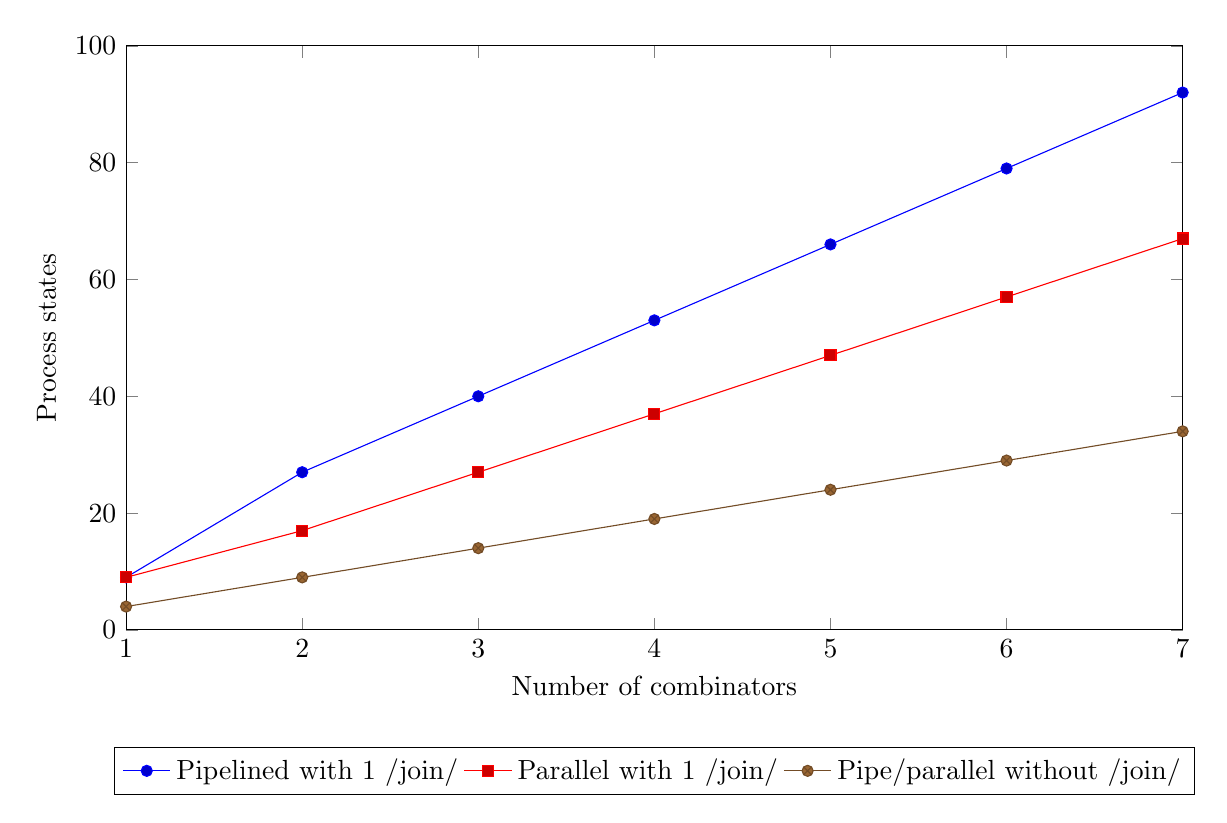
\begin{tikzpicture}
\begin{axis}[
% Hide the label on the second graph
	ylabel=Process states,
	xlabel=Number of combinators,
  ymin=0, ymax=100,
  xmin=1, xmax=7,
  xtick=data,
    width=15cm, height=9.0cm,
    legend style={at={(0.5,-0.2)},anchor=north, legend columns=4},
]
\addplot coordinates {(1,9) (2,27) (3,40) (4,53) (5,66) (6,79) (7,92) };
\addplot coordinates {(1,9) (2,17) (3,27) (4,37) (5,47) (6,57) (7,67) };
\addplot coordinates {(1,4) (2,9) (3,14) (4,19) (5,24) (6,29) (7,34)  };

\legend{Pipelined with 1 \Hs/join/, Parallel with 1 \Hs/join/, Pipe/parallel without \Hs/join/};
\end{axis}
\end{tikzpicture}

\caption{Maximum output process size for fusing all combinations of up to $n$ combinators}
\label{fig:bench:outputsize}
\end{figure}


% -----------------------------------------------------------------------------
\begin{figure}

\begin{tikzpicture}
\begin{axis}[
	ylabel=Process states,
	xlabel=Number of \Hs/join/ combinators,
%  ymode=log,
  ymin=0, ymax=1500,
	enlargelimits=0.01,
  xtick=data,
  xmin=1, xmax=7,
    width=15cm, height=9.0cm,
	legend pos=north west,
]
% These are the values for splitting.
% They are smaller than the 'chaining', but look much nicer on the linear graph.
\addplot coordinates {(1,9) (2,42) (3,97) (4,196) (5,383) (6,746) (7,1461) (8,2880) };

% These are the values for chaining
% \addplot coordinates {(1,4) (2,48) (3,194) (4,760) (5,2814) (6,10064) (7,1) };

\end{axis}
\end{tikzpicture}

\caption{Exponential blowup occurs when splitting or chaining \Hs/join/ combinators together}
\label{fig:bench:exponential}
\end{figure}



The size of the result process is roughly what one would get when inlining the definitions of each of the original source processes. This is common with other systems based on inlining and/or template meta-programming, and is not prohibitive.

On the other hand, \cref{fig:bench:exponential} shows the results for a pathological case where the size of the output program is exponential in the number of input processes. The source dataflow networks consists of N join processes, N+1 input streams, and a single output stream. The output of each join process is the input of the next, forming a chain of joins. In source notation the network for N = 3 is (\Hs@sOut = join sIn1 (join sIn2 (join sIn3 sIn4))@).

When fusing two processes, the fusion algorithm essentially compares every state in the first process with every state in the second, computing a cross product. During the fusion transform, as states in the result process are generated they are added to a finite map --- the \Hs@instrs@ field of the process definition. The use of the finite map ensures that identical states are always combined, but genuinely different states always make it into the result. 

In the worst case, fusion of two processes produces O($n*m$) different states, where $n$ and $m$ are the number of states in each. If we assume the two processes have about the same number of states then this is O($n^2$). Fusing the next process into this result yields O($n^3$), so overall the worst case number of states in the result will be O($n^k$), where $k$ is the number of processes fused. 

In the particular case of \Hs@join@, the implementation has two occurrences of the \Hs@push@ instruction.
During fusion, the states for the consuming process are inlined at each occurrence of \Hs@push@.
These states are legitimately different because at each occurence of \Hs@push@ the input channels of the join process are in different channel states, and these channel states are included in the overall process state.
It may be possible to solve this problem by introducing the concept of subroutines, which would allow the same set of consumer instructions to be reused by the different occurences of the \Hs/push/ instructions.
The fusion algorithm would be modified to inline the definition of a subroutine when required to coordinate between the two processes; when coordination is not required, the subroutine can be called as-is.
Currently, all instructions are continuation-passing-style and the processes do not require a call-stack.
To ensure subroutines can be executed with a statically bounded call-stack, subroutines must be non-recursive, but it may be possible to allow subroutines to perform loops and call other subroutines.

\section{Conclusion}
In the benchmarks, we saw that Folderol was always competitive with the hand-fused program, and in all but a few cases, faster than the other programs.
For array computations there is some extra code required to convert between vectors and streams.
There is also some extra wrapping with Template Haskell splices and quasiquotes, but this is fairly minor, and the required changes are more or less mechanical and type-driven.

Another benefit, aside from performance, is not having to inspect the compiler's intermediate representation or generated code to know whether whether fusion has worked or failed.
If fusion succeeds, we know it has succeeded.
If fusion fails, we are told which parts of the process network were able to be fused, and which parts were not.
These explicit fusion failures make it significantly easier to track down performance issues due to non-fusion.

